
\chapter{Methods}




\section{Neuron and network model}

This section will go into detail about the dendritic error network \citep{sacramento2018dendritic}. The model contains a
somewhat complex and strongly recurrent connectivity, which poses one of the major criticisms aimed at it
\citep{whittington2019theories}. Much like traditional machine learning networks, it can be functionally separated into
layers. Yet in this particular model, input- hidden- and output layers are quite distinct in both neuron populations and
connectivity.


\subsection{Network architecture}

\begin{figure}[t]
  \centering
  \begin{minipage}{0.5\textwidth}
    \centering
    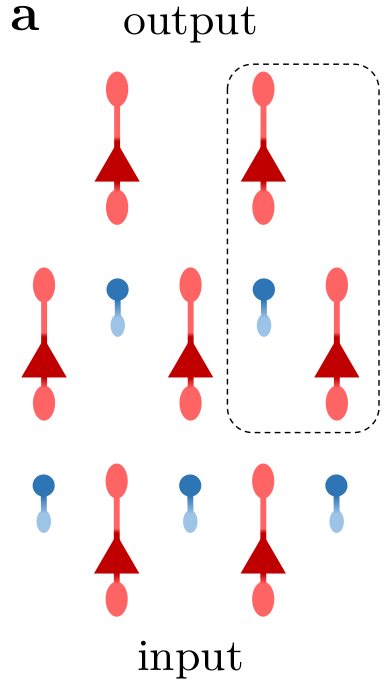
\includegraphics[width=0.9\textwidth]{network_a}
  \end{minipage}\hfill
  \begin{minipage}{0.4\textwidth}
    \centering
    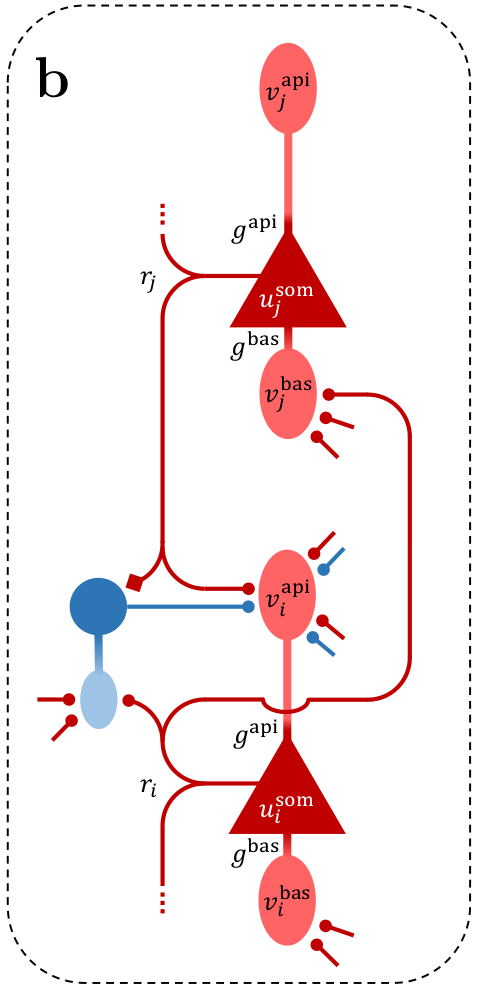
\includegraphics[width=0.9\textwidth]{network_b}
  \end{minipage}
  \caption{Network structure, from \cite{Haider2021}. \textbf{a:} pyramidal- (red) and interneurons (blue) in a network
    of three layers. Note the fact that the number interneurons in a layer is equal to the number of pyramidal neurons
    in the subsequent layer\protect\footnotemark. \textbf{b:} connectivity within the highlighted section. Feedback
    pyramidal-to-interneuron connections (displayed with rectangular synapse) transmit pyramidal somatic potential
    directly and connect to a single interneuron. This enables these interneurons to learn to match their corresponding
    next-layer pyramidal neurons. All other synapses (circles) transmit the neuron somatic activation $\phi (u^{som})$
    and fully connect their origin and target populations.}
  \label{fig-network}
\end{figure}

\footnotetext{{Note that the input layer is displayed as having interneurons here. This appears to be a mistake in the
      Figure. Within the implementation, interneurons are only modelled in hidden layers.}}

The basic connectivity scheme of the Model is shown in Figure \ref{fig-network}. Neurons at the input layer receive no
feedback signals and serve primarily to apply a temporals low-pass filter to the stimulus which is injected directly
into their membrane.  Hidden layers consist of a pyramidal- and an interneuron population, which are fully connected to
each other reciprocally. Both types of neurons are represented by multi-compartment neuron models with leaky membrane
dynamics. Interneurons contain one somatic and one dendritic compartment, while pyramidal neurons are modeled with both
a basal and an apical dendrite (cf. Section \ref{sec-neurons}).  Feedforward connections between layers are facilitated
by all-to-all connections between their respective pyramidal neurons and innervate basal compartments. Hidden layer
pyramidal neurons additionally connect to all interneurons within their layer. Feedback connections from superficial
pyramidal neurons and lateral interneurons on the other hand arrive at apical compartments of pyramidal neurons. Thus, a
hidden layer pyramidal neuron forms two reciprocal loops, one with all interneurons in the same layer, and one with all
pyramidal neurons in the next layer.

Hidden layer interneurons receive feedback information from superficial pyramidal neurons in addition to their lateral
connections. These feedback connections are special, since they connect one pyramidal neuron to exactly one interneuron.
Instead of transmitting a neuronal activation $\phi(u_{l+1}^P)$ as all other connections do, these connections relay
somatic voltage $u_{l+1}^P$ directly. This one-to-one connectivity puts a strict constraint on the number of
interneurons in a hidden layer, as it must match the number of subsequent pyramidal neurons. These pairs of inter- and
pyramidal neurons that have matching somatic activations will henceforth be called \textit{sister neruons}. Their
connections serve to \textit{nudge} interneuron somatic activation towards that of their pyramidal sisters. The purpose
of an interneuron in this architecture is then, to predict the activity of its sister neuron. Any failure to do so
results in layer-specific errors which in turn are the driving force of learning in this context, but more on this
later.  The connectivity between them share features of electrical synapses, which will be discussed in Section
\ref{sec-electric-syns}. \todo{keep last sentence?}


Output layers have no interneurons, and are usually modeled as pyramidal neurons without an apical compartment. During
learning, the target for the network's activation is injected into their somatic compartment. Through the feedback
connections, it can propagate through the entire network. To understand what purpose this rather complex connectivity
scheme serves in our model, neuron models and plasticity rules require some elaboration.


\subsection{Neuron models}\label{sec-neurons}



The network contains two types of multi-compartment neurons; Pyramidal neurons with three compartments each, and
interneurons with two compartments each. They integrate synaptic inputs into dendritic potentials, which in turn leak
into the soma with specific conductances. Note that vector notation will be used throughout this section, and $u_l^P$
and $u_l^I$ denote the column vectors of pyramidal- and interneuron somatic voltages at layer $l$ respectively. Synaptic
weights $W$ are likewise assumed matrices of size $n \times m$, which are the number of output and input neurons of the
connected populations respectively. The activation $r_l^P$ of pyramidal neurons is given by applying the synaptic
transfer function $\phi$ to to their somatic potentials $u_l^P$:
\begin{align}
  r_l^P   & = \phi(u_l^P)                                                                      \\
  \phi(x) & = \begin{cases}
                0                                   & \textrm{if } \ x < -\epsilon               \\
                \gamma \ log(1+e^{\beta(x-\theta)}) & \textrm{if } \ -\epsilon \leq x < \epsilon \\
                \gamma \ x                          & \textrm{otherwise}
              \end{cases}
\end{align}

where $\phi$ acts componentwise on $u$ and can be interpreted as a smoothed variant of ReLu (sometimes called
\textit{Softplus}) with scaling factors $\gamma=1$, $\beta=1$, $\theta=0$. Splitting the computation with the threshold
parameter $\epsilon=15$ does not change its output, but instead serves to prevent overflow errors for large absolute
values of $x$.

As mentioned before, pyramidal and interneurons are modeled as rate neurons with leaky membrane dynamics and multiple
compartments. Where applicable, they will be differentiated with superscripts $P$ and $I$ respectively. The basal and
apical dendrites of pyramidal neurons are denoted with superscripts $bas$ and $api$ respectively, while interneuron
dendrites are simply denoted $dend$.  The derivative somatic membrane potentials of layer $l$ pyramidal neurons is given by:

\begin{align}
  C_m \dot{u}_l^P & = - g_l u_l^{P} + g^{bas} v_l^{bas} + g^{api} v_l^{api} \label{eq-pyr-dynamics-rate}
\end{align}

where $g_l$ is the somatic leakage conductance, and $C_m$ is the somatic membrane capacitance, which will be assumed to
be $1$ from here on out. $v_l^{bas}$ and $v_l^{api}$ are the membrane potentials of basal and apical dendrites
respectively, and $g^{bas}$ and $g^{api}$ their corresponding coupling conductances.  Dendritic compartments in this
model have no persistence between simulation steps. Thus, they are defined at every timestep $t$ through incoming weight
matrices and presynaptic activities:

\begin{align}
  v_l^{bas}(t) & = W_l^{up} \ \phi(u_{l-1}^P(t)) \label{eq-v-bas-rate}                                     \\
  v_l^{api}(t) & =  W_l^{pi} \ \phi(u_l^I(t)) \ + \  W_l^{down} \ \phi(u_{l+1}^P(t)) \label{eq-v-api-rate}
\end{align}

The nomenclature for weight matrices conforms to \cite{Haider2021}, where weight matrices are indexed by the layer in
which their neurons terminate and belong to one of four populations: Feedforward and feedback pyramidal-to-pyramidal
connections arriving at layer $l$ are denoted $W_l^{up}$ and $W_l^{down}$ respectively. Lateral pyramidal-to-interneuron
connections are denoted with $W_l^{ip}$ and their corresponding feedback connections with $W_l^{pi}$.
\newline

Interneurons integrate synaptic information by largely the same principle, but instead of top-down signals from their
sister neurons arriving at an apical compartment, it is injected directly into the soma. Through this, interneurons
functionally resemble the original two-compartment neuron from \cite{urbanczik2014learning} most closely.

\begin{align}
  C_m \dot{u}_l^I & = - g_l u_l^{I} + g^{dend} v_l^{dend} + i^{nudge, I}\label{eq-intn-dynamics} \\
  i^{nudge, I}    & = g^{nudge, I} u_{l+1}^P                                                     \\
  v_l^{dend}      & = W_l^{ip} \ \phi(u_{l}^P)
\end{align}

where $ g^{nudge, I}$ is the interneuron nudging conductance, and $u_{l+1}^P$ is the somatic voltage of pyramidal
neurons in the next layer.  Pyramidal neurons in the output layer $N$ effectively behave like interneurons, as they
receive no input to their apical compartment. Instead, the target  activation $u^{tgt}$ is injected into their soma:

\begin{align}
  C_m \dot{u}_N^P & = - g_l u_N^{P} + g^{bas} v_N^{bas} + i^{nudge, tgt} \\
  i^{nudge, tgt}  & = g^{nudge, tgt} u^{tgt}
\end{align}


These neuron dynamics correspond closely to those by \cite{urbanczik2014learning}, including the extension to more than
two compartments which was proposed in the original paper. It should be noted however, that they are simplified in some
ways. For example, dendritic couplings and nudging are not relative to the somatic or some reversal potential (i.e.
$i^{nudge, tgt}= g^{nudge, tgt} (u^{tgt} - u_N^P )$), but are only dependent on absolute currents. Additionally, the
strict separation of excitatory and inhibitory synaptic integration (cf. Section \todo{write about this}), as well as
additional nonlinearities in the plasticity are omitted.  These simplifications do increase computational speed and
allow for a much simpler approximation of network dynamics via a steady-state. Yet they do come at the cost of omitting
neuroscientific insights from the model, which I view critically. \phrasing




\section{Urbanczik-Senn Plasticity}\label{sec-urb-senn-plast}

The synapses in the network are all modulated according to variations of the "Urbanczik-Senn" plasticity rule
\citep{urbanczik2014learning}, which will be discussed in this section. After detailing the (simplified) weight update,
I will briefly discuss the scientific significance of the plasticity model.

\subsection{Derivation}

The plasticity rule is only defined for postsynaptic neurons which have one somatic and at least one dendritic
compartment, to the latter of which synapses with this plasticity can connect. Functionally, synaptic weights are
changed in such a way, as to minimize discrepancies between somatic and dendritic potential. This discrepancy is called
the \textit{dendritic error}. The change in weight for a synapse fron neuron $j$ to the basal compartment of a pyramidal
neuron $i$ is given by:

\begin{align}
  \dot{w}_{ij}    & = \eta \ ( \phi(u_i^{som}) - \phi(\hat{v}_i^{bas}) ) \ \phi(u_j^{som})^T \\
  \hat{v}_i^{bas} & = \alpha \  v_i^{bas}
\end{align}

with learning rate $\eta$, and $u^T$ denoting the transposition of the vector $u$ (which is by default assumed a column
vector). The dendritic prediction $\hat{v}_i^{bas}$ is a scaled version of the dendritic potential by the constant
factor $\alpha$, which is calculated from coupling and leakage conductances. As an example, basal dendrites of pyramidal
neurons in \cite{sacramento2018dendritic} are attenuated by $\alpha = \frac{g^{bas}}{g_l + g^{bas} + g^{api}}$. A key
property of this value for $\alpha$ is, that dendritic error is $0$, when the only input to a neuron stems from the
given dendrite. In other words, the dendrite predicts somatic activity perfectly. Neuron- and layer-specific differences
in $\alpha$, as well as an analytical derivation are detailed in \citep{sacramento2018dendritic}.

If a current is injected into the soma (or in this case, into a different dendrite), a dendritic error arises, and
plasticity drives synaptic weights to minimize it. In addition to the learning rate $\eta$, $\dot{w}_{ij}$ scaled by the
presynaptic activity $\phi(u_j^{som})$. Therefore, a dendritic error arising without presynaptic contribution does not
elicit a change in that particular synapse.  
Updates for the weight matrices in a hidden layer $l$ of the present network model are given by:

\begin{align}
  \dot{w}_{l}^{up}   & = \eta_l^{up} \ ( \phi(u_l^{P}) - \phi(\hat{v}_l^{bas}) ) \ \phi(u_{l-1}^{P})^T\label{eq-delta_w_up}         \\
  \dot{w}_{l}^{ip}   & = \eta_l^{ip} \ ( \phi(u_l^{I}) - \phi(\hat{v}_l^{dend}) ) \ \phi(u_{l}^{P})^T\label{eq-delta_w_ip}          \\
  \dot{w}_{l}^{pi}   & = \eta_l^{pi} \ - v_l^{api} \ \phi(u_l^{I})^T\label{eq-delta_w_pi}                                           \\
  \dot{w}_{l}^{down} & = \eta_l^{down} \ ( \phi(u_l^{P}) - \phi(w_l^{down} r_{l+1}^P) )\ \phi(u_{l+1}^{P})^T\label{eq-delta_w_down}
\end{align}

Each set of connections is updated with a specific learning rate $\eta$ and a specific dendritic error term. The purpose
of these error terms will be explained in Section \ref{sec-selfpred}. Note that pyramidal-to-pyramidal feedback weights
$w_l^{down}$ are not plastic in the present simulations and are only listed for completeness, see Section
\ref{sec-feedback-plast}.


\subsection{Neuroscientific significance}

\todo{this is going to be hard}

Dendritic plateau potentials

\todo{Dendritic spikes}

\section{The self-predicting network state}\label{sec-selfpred}

In this model, euron dynamics, plasticity rules and network architecture form an elegant interplay, which I expand on in
this section. We will

Since each interneuron receives a somatic nudging signal from its corresponding next-layer pyramidal neuron, incoming
synapses from lateral pyramidal neurons adapt their weights to match feedforward pyramidal-to-pyramidal weights. In
intuitive terms; Feedforward pyramidal-to-pyramidal weights elicit a certain activation in the subsequent layer, which
is fed back into corresponding interneurons. In order to minimize the dendritic error term in Equation
\ref{eq-delta_w_ip}, pyramidal-to-interneuron weight matrices at every layer must match these forward weights ($w_l^{ip}
\approx \rho w_l^{up}$) up to some scaling factor $\rho$. $\rho$ depends on the difference in parameters between
pyramidal- and interneurons, and is close to $1$ for most of the simulations considered here. As long as no feedback
information arrives at the pyramidal neurons, the Urbanczik-Senn plasticity drives synaptic weight to fulfill this
constraint. Note, that this alignment of two separate sets of outgoing weights is acheived with only local information.
Therefore this mechanism could plausibly align the weights of biological synapses that are physically separated by long
distances. \newline

Next, consider the special case for interneuron-to-pyramidal weights in Equation \ref{eq-delta_w_pi}, in which
plasticity does not serve to reduce discrepancies between dendritic and somatic potential. The error term is instead
defined solely by the apical compartment voltage\footnote{In strict terms, it is defined by the deviation of the
dendritic potential from its specific reversal potential. Since that potential is zero throughout, $- v_l^{api}$ remains
as the error term.}. Thus, plasticity in these synapses works towards silencing the apical compartment. The apical
compartments also receive feedback from superficial pyramidal neurons, whose synapses will be considered non-plastic for
now. As shown above, interneurons each learn to match their respective sister neuron activity. Thus, silencing of apical
compartments can only be acheived by mirroring the pyramidal-to-pyramidal feedback weights ($w_l^{pi} \approx
-w_l^{down}$).\newline

When enabling plasticity in only these two synapse types, the network converges on the "\textbf{self-predicting state}"
\citep{sacramento2018dendritic}. This state is defined by a minimization of four error metrics at each hidden layer $l$:

\begin{itemize}
  \item The symmetries between feedforward ($w_l^{ip} \approx \rho w_l^{up}$) and feedback ($w_l^{pi} \approx
          -w_l^{down}$) weights. Mean squared error between these pairs of matrices will be called \textbf{Feedforward -
          } and \textbf{Feedback weight error} respectively.
  \item Silencing of pyramidal neuron apical compartments ($v_l^{api} \approx 0$). The Frobenius norm \citeme of apical
        compartment voltages within a layer is called the \textbf{Apical error}.
  \item Equal activations in interneurons and their respective sister neurons ($\phi (u_l^I) \approx \phi (u_{l+1}^P)$).
        The mean squared error over these vectors is called the \textbf{Interneuron error}.
\end{itemize}

\what{is there a mathematical symbol for this type of convergence?}

All of these equalities are approximate, since the network does not ever reach a state in which all of these values are
zero. In the original implementation, these deviations are minute and can likely be explained with floating point
conversions. Since it is impossible to replicate the timing of the original precisely within NEST, the NEST simulations
deviate more strongly from this ideal. The key insight here is, that this state is not clearly defined by absolute error
thresholds, but is rather flexible. Thus, networks are able to learn successfully even when their weights are
initialized imperfectly. \todo{or not at all? some science is required here}

An analysis of the equations describing the network reveals that the self-predicting state is stable \phrasing. When
Interneuron error is zero, dendritic and somatic compartments of all interneurons are equal, thus effectively disabling
plasticity in incoming synapses. Likewise, a silenced apical compartment will disable plasticity in all incoming
synapses. Synapses from lateral interneurons (Equation \ref{eq-delta_w_pi}) only depend on the apical compartment
itself, thus can not change in this state. Similarly, the apical compartment is also the driving factor for the
dendritic error of feedforward synapses (Equation \ref{eq-delta_w_up}), since it affects somatic activity when
active\footnote{This feature is actually rather important when contemplating biological neurons using the Urbanczik-Senn
plasticity. In the original paper, currents were injected directly into the soma to change the error term. The the
introduction of a second dendrite which performs that very task is much more useful, as originally described by the
authors. Whether interneurons could be modeled by the same principles will be discussed in Section \todo{talk about
interneuron dendritic trees}}. Thus, all plasticiy in the network is disabled, and remains in the self-predicting state
regardless of the kind of stimulus injected into the input layer. This fact highlights another important property of
networks in this state. Notice, how information flows backwards through the network; All feedback signals between layers
ultimately pass through the apical compartments of pyramidal neurons. Thus, successful silencing of all apical
compartments implies that no information can travel backwards between layers (with the exception of interneurons
receiving top down signals). As a result, the network behaves strictly like a fully connected feedforward network
consisting only of pyramidal neurons. The recurrence within this network is in balance, and completely cancels out its
own effects. This holds true as long as all conditions for the self-predicting state are fulfilled, and the network only
receives external stimulation at the input layer. One interpretation of this is, that the network has learned to predict
its own top-down input. A failure by interneurons to fully explain (i.e. cancel out) top-down input thus results in a
prediction error, encoded in deviation of apical dendrite potentials from their resting state. This prediction error in
turn elicits plasticity in all synapses connecting to its pyramidal neuron, which drives the network towards a
self-predicting state that is congruent with the novel top-down signal. Therefore, these neuron- specific prediction
errors are the driving force of supervised learning in these networks



\section{Training the network}

Starting with a network in the self-predicting state, performing time-continuous supervised learning then requires an
injection of a target activation into the network's output layer alongside with a stimulus at the input layer. Since
output layer neurons feed back into both interneurons and pyramidal neurons of the previous layer, local prediction
errors arise. Synapses activatee and drive to minimize the prediction errors, which requires the network to replicate
the target activation from activations and weights of the last hidden layer.

Note, that this mechanism is not exclusive to the last two layers. Any Apical errors cause a change in somatic activity,
which previous layers will fail to predict. Thus, errors are propagated backwards through the entire network, causing
error minimization at every layer. See the Supplementary analysis of \cite{sacramento2018dendritic} for a rigorous proof
that this type of network does indeed approximate the Backpropagation algorithm \what{what does the $\mathit{O}$ mean?}.



Classical backpropagation relies on a strict separation of a forward pass of some stimulus, and subsequent a backwards
pass dependent on the arising loss at the output layer. Since the present network is time-continuous, stimulus and
target activation are injected into the network simultaneously. These injections are maintained for a given presentation
time $t_{pres}$, in order to allow the network to calculate errors through its recurrent connections before slowly
adapting weights. Particluarly for deep networks, signals travelling from both the input and output layer require some
time to balance out and elicit the correct dendritic error terms. This property poses the most significatn drawback of
this type of time-continuous approximation of Backpropagation: The network tends to overshoot activations in some
neurons, which in turn causes an imbalance between dendritic and somatic compartments. This effect causes the network to
change synaptic weights away from the desired state during the first few miliseconds of a stimulus presentation. The
solution Sacramento et al. found for this issue was to drastically reduce learning rates, while increasing stimulus
presentation time. This solution is sufficient to prove that plasticity in this kind of network is able to perform error
propagation, but still has some issues. Most notably, training is highly inefficient and computationally intensive. A
closer investigation of the issue as well as a solution will be discussed in Section \ref{sec-haider}.



\section{The NEST simulator}

One of the key research questions motivating this thesis is whether the network would be able to learn successfully when
employing spike-based communication instead of the rate neurons for which it was developed. As a framework for my
spike-based implementation two options were considered: The first one was to use the existing implementation of the
network which employs \texttt{PyTorch} and \texttt{NumPy}, and expand it to employ spiking neurons. PyTorch does in
principle support spiking communication between layers, but is streamlined for implementing less recurrent and less
complex network and neuron models. Another concern is efficiency; PyTorch is very well optimized for efficiently
computing matrix operations on dedicated hardware. This makes it a good choice for simulating large networks of rate
neurons, which transmit all of their activations between layers at every simulation step. Spiking communication between
leaky neurons is almost antithetical to this design philosophy and thus can be expected to perform comparatively poor
when using this backend.

The second option was to use the NEST simulator
(\href{https://nest-simulator.readthedocs.io}{nest-simulator.readthedocs.io}), which was developed with highly parallel
simulations of large spiking neural networks in mind. It is written in C++ and uses the \textit{Message Passing
Interface} (\href{https://www.mpi-forum.org/}{MPI}) to efficiently communicate evends between both threads and compute
nodes. One design pillar of the simulator, which is particularly relevant for this project, is the event-based
communication scheme that underpins all simulated nodes. It ensures that communication bandwidth at every simulation
step is only used by the subset of nodes which transmit spikes or other signals at that time step. Yet the most notable
advantage of the NEST simulator is, that an event-based implementation of the Urbanczik-Senn plasticity alongside a
corresponding neuron model had already been developed for it. Combined with the fact that I had more prior experience
with NEST over PyTorch, I decided to implement the spiking neuron model in the NEST simulator.

The simulator has one particular limitation which needs to be considered. As communication between compute nodes takes
time, Events\footnote{An Event in NEST is an abstract C++ Class that is created by neurons, and transmitted across
threads and compute nodes by the Simulator. A Multitude of Event types are provided (i.e. \texttt{SpikeEvent,
CurrentEvent, RateEvent}), each able to carry specific types of payload and being processed differently by postsynaptic
neurons.} can not be handled in the same simulation step in which they were sent. Thus, NEST enforces a synaptic
transmission delay of at least one simulation step for all connections. This property is integral to many parallel
simulation backends \citep{davies2018loihi,Hines1997,Schepper2022}, and is in line with synaptic delays of biological
neurons. Yet particularly with regard to network relaxation, it can be expected to affect performance.


\section{Transitioning to spiking communication}

The spiking neuron models rely heavily on the model from \citep{Stapmanns2021}, in which it was shown that spiking
neurons are able to perform learning tasks that were designed for the rate neurons described in
\cite{urbanczik2014learning}. The existing model is an exact replication of the Urbanczik-Senn neuron in terms of
membrane dynamics. The critical update of that model is that instead of transmitting their hypothetical rate $r =
\phi(u)$ at every time step, these neurons emit spikes in a similar way to stochastic binary neurons
\citep{Ginzburg1994}. The number of spikes to be generated during a simulation step $n$ is determined by drawing from a
Poisson distribution, which takes $r$ as a parameter:

\begin{align}
  P\{\textit{n} \ \text{spikes during} \ \Delta t\} & = e^{-r \Delta t} \frac{(r \ \Delta t) ^ n}{n!}\label{eq-pr-n-spikes} \\
  \langle \textit{n} \rangle                        & = r \ \Delta t \label{eq-n-spikes}
\end{align}

\todo{find a citation for this}

where $\Delta t$ denotes the integration time step of the simulator, which will be assumed to be $0.1 ms$ from here on
out.  $\langle \textit{n} \rangle$ denotes the expected number of spikes to be emitted in a simulation step, i.e.
between $[t, t+ \Delta t]$. Note that this mechanism makes the assumption that more than one spike can occur per
simulation step. NEST was developed with this possibility in mind and provides a \textit{multiplicity} parameter for
Spike Events, which is processed at the postsynaptic neuron. As the high spike frequencies resulting from this could not
occur in biological neurons, the model is also capable of simulating a refractory period. For this, the number of spikes
per step is limited to $1$, and the spiking probability is set to 0 for the duration of the refractory period $t_{ref}$.
The probability of at least one spike occuring within the next simulation step is given the inverse probability of no
spike occuring. Thus, when inserting $n=0$ into Equation \ref{eq-pr-n-spikes}, the probability of eliciting at least one
spike within the next simualtion step can be derived as:

\begin{align}
  P\{ \textit{n} \geq 1\} & = 1 - e^{-r \Delta t}
\end{align}


Drawing from this probability then determines whether or not a spike is sent during that step, henceforth denoted with
the function $s(t)$, which outputs $1$ if a spike is sent during the interval $[t, t+\Delta t]$ \todo{Notation
correct?}, and $0$ otherwise. \newline

In order to implement the plasticity rule for spiking neurons, dendritic compartments need to be modeled with leaky
dynamics. These dynamics are fundamentally the same as those described for the somatic compartment. Thus, the dendritic
compartment of neuron $j$ evolves according to:

\begin{align}
  C_m^{bas} \dot{v}_j^{bas} & = -g_l^{bas} \  v_j^{bas} + \sum_{i \in I} W_{ji} s_i(t)     \label{eq-spiking-basal-compartment}
\end{align}

with presynaptic neurons $I$, and membrane capacitance $C_m^{bas}$ and leakage conductance $g_l^{bas}$ being specific to
the basal dendrite. Note that these equations are calculated individually for each neuron and do not employ the matrix
notation used for layers of rate neurons. Pyramidal apical and interneuron dendritic compartments evolve by the same
principle and with largely the same parameters.

\section{Event-based Urbanczik-Senn plasticity}\label{sec-event-urb}

One major challenge in implementing this architecture with spiking neurons is the Urbanczik-Senn plasticity introduced
in Section \ref{sec-urb-senn-plast}. Since the plasticity rule is originally defined for rate neurons, computing the
updates for spiking neurons requires some additional effort. Fortunately, this problem has already been solved in NEST
for two-compartment neurons \citep{Stapmanns2021}. This Section will discuss its algorithm and implementation. \newline

Since NEST is an event-based simulator, most of the plasticity mechanisms developed for it compute weight changes at the
location (i.e. thread and compute node) of the postsynaptic neuron whenever an Event is received. This has several
advantages; It allows the thread that created the Event to continue processing neuron updates instead of having to
synchronize with all threads that manage recipient neurons.  More importantly, this feature mirrors the local properties
of biologically synaptic plasticity models, as these are often considered to be dependent on factors that are local to
the synapse \citeme. For a spiking implementation of the Urbanczik-Senn plasticity, dendritic errors at every time step
are required instead of just a scalar trace at the time of a spike, as would be the case for STDP. Thus, a mechanism for
storing and reading these errors was requred, for which two basic possibilities were considered:

In a \textbf{Time-driven scheme}, dendritic errors are made available to synapses at every timestep, and weight changes
are applied instantaneously. This approach requires very little memory, as no history of dendritic errors needs to be
stored. It does come at the cost of computational efficiency, since calls to the synaptic update function are as
frequent as neuron updates - for all synapses. Particularly for large numbers of incoming synapses, as is common for
simulations of cortical pyramidal neurons \citep{potjans2014cell,vezoli2004quantitative}, this implies a large number of
function calls per time step. It also means that weight changes need to be computed at time steps where they are not
immediately required (i.e. when there is no presynaptic activity), or when no weight change is necessary. Therefore,
this approach proved costly in terms of Computational resources.

An \textbf{Event-driven scheme} on the other hand, updates synaptic weights only when a spike is sent through the
synapse. A history of the dendritic error is stored at the postsynaptic neuron, which is read by each synapse when a
spike is transmitted in order to compute weight changes. As the history of dendritic error applies equally to all
incoming synapses, it only needs to be recorded once at the neuron. Alongside each entry in the history, a counter is
stored and incremented whenever a synapse has read the history at that time step. Once all synapses have read out an
entry, it is deleted. Thus, the history dynamically grows and shrinks during simulation and is only ever as long as the
largest inter-spike interval (ISI) of all presynaptic neurons. This approach proves to be more efficient in terms of
computation time, since fewer calls to the update function are required per synapse. It does come at the cost of memory
requirements, as the history can grow particularly large for simulations with low in-degrees or large ISI\footnote{It
should also be noted that in this approach requires redundant integration of the history by every synapse. Stapmanns et
al. propose a third solution, in which this integration is performed once whenever a spike is received, with the
resulting weight change being applied to all synapses immediately. This approach proved to be even more efficient for
some network configurations, but is incompatible with simulations where incoming synapses have heterogeneous synaptic
delays due to the way that these delays are processed by the NEST simulator. See Section 3.1.3 in \cite{Stapmanns2021}
for a detailed explanation.}. During testing, the Event-based schemed proved substantially more efficient for many
network types. This did however introduce the challenge of retroactively computing weight changes from the time of the
last spike upon arrival of a new spike. \newline


\subsection{Integrating weight changes}


Stapmanns et al. describe the Urbanczik-Senn plasticity rule based on the general form for weight changes

\begin{align}
  \dot{w}_{ij}(t) & = F(s_j^\ast (t), V_i^\ast (t)) \label{eq-delta-w-spiking}
\end{align}

where the change in weight $\dot{w}_{ij}$ of a synapse from neuron $j$ to neuron $i$ at time $t$ is given by a function
$F$ that depends on the dendritic error of the postsynaptic neuron $V_i^\ast$ and the presynaptic spiketrain $s_j^\ast$.
The $\ast$ operator denotes a causal function, indicating that a value $V_i^\ast(t)$ potentially depends on all previous
values of $V_i(t' < t)$. One can formally integrate Equation \ref{eq-delta-w-spiking} in order to obtain the weight
change between two arbitrary time points $t$ and $T$:

\begin{align}
  \Delta w_{ij}(t,T) & = \int_t^T dt' F[s_j^\ast, V_i^\ast](t') \label{eq-delta-w-t-T}
\end{align}

This integral is of forms the basis of computing the change in weight between two arriving spikes. Thus, at the
implementational level, $t$ is usually the time of the last spike that traversed the synapse, and $T$ is the current
\texttt{biological\_time}\footnote{This term is adopted from the NEST convention, where it describes the time for which
a neuron or network has been simulated in $ms$. It describes how many simulation steps of length $\Delta t \ ms$ have
been computed, and is therefore independent from a simulation's runtime  on the employed hardware (also called
\textit{wall clock time} \citep{albada2018performance}). }. For spiking neurons, it is necessary to approximate the
presynaptic activation ($\phi(u_j)$). For this, a well established solution is to transform the spiketrain $s_j$ into a
decaying trace using an exponential filter kernel $\kappa$:

\begin{align}
  \kappa(t)     & = H(t) \frac{1}{t}e^{\frac{-t}{\tau_{\kappa}}}                        \\
  H(t)          & =
  \begin{cases}
    1 & \text{if $t > 0$}    \\
    0 & \text{if $t \leq 0$} \\
  \end{cases}                                                              \\
  (f \ast g)(t) & = \int_{- \infty }^{\infty} f(t') g(t-t') d t' \label{eq-convolution} \\
  s_j^\ast      & = \kappa_s \ast s_j. \label{eq-spike-trace}
\end{align}

with filter time constant $\tau_\kappa$. To obtain the trace of a spiketrain, it is convolved (Equation
\ref{eq-convolution}) with the exponential filter kernel $\kappa$. The filter uses the Heaviside step function $H(t)$,
and is therefore only supported on positive values of $t$ (also called a one-sided exponential decay kernel). This
property is important, as integration limits of the convolution can be truncated when $f$ and $g$ are both only
supported on $[0,\infty)$:

\begin{align}
  (f \ast g)(t) & = \int_{0}^{t} f(t') g(t-t') d t'
\end{align}

Since spikes naturally only occur at $t>0$, this simplified integral allows for a much more efficient computation of the
spike train. In this particular case, the Function $F$ on the right hand side of Equation \ref{eq-delta-w-spiking} is
defined as:

\begin{align}
  F[s_j^\ast, V_i^\ast] & = \eta \kappa \ast (V_i^\ast s_j^\ast)        \\
  V_i^\ast              & = (\phi(u_i^{som}) - \phi(\hat{v}_i^{dend}) )
\end{align}

\what{this notation seems slightly abusive but is taken precisely from \cite{Stapmanns2021}} with learning rate $\eta$.
$V_i^\ast$ then is the dendritic error of the dendrite that the synapse between $j$ and $i$ is located at\footnote{The
dendritic error here is defined as the difference between two hypothetical rates based on the arbitrary function $\phi$.
The original implementation uses the difference between the actual postsynaptic spiketrain and this dendritic prediction
($V_i^\ast = (s_i - \phi(\hat{v}_i^{dend}) )$). Furthermore, Stapmanns et al. show that generating a spiketrain from the
dendritic potential ($V_i^\ast = (s_i - s_i^{dend})$) also results in successful learning, although at the cost of
additional training time. This variant was chosen in order to not decrease learning performance any more than
necessary.}. Writing out the convolutions in Equation \ref{eq-delta-w-t-T} explicitly, we obtain

\begin{align}
  \Delta w_{ij}(t,T) & = \int_t^T dt' F[s_j^\ast, V_i^\ast](t')                                                                           \\
                     & =  \int_t^T dt' \  \eta\int_0^{t'} dt'' \ \kappa(t'-t'') V_i^\ast (t'') s_j^\ast (t'') \label{eq-delta-w-t-T-long}
\end{align}

Computing this Equation directly is computationally inefficient due to the nested integrals. Yet, it is possible to
break up the integrals into two simpler computations and rewrite the weight change as:


\begin{align}
  \Delta W_{ij}(t, T) & = \eta \left[ I_1 (t, T) - I_2(t,T) + I_2(0,t)\left( 1- e^{-\frac{T-t}{\tau_\kappa}} \right) \right] \\
  I_1(a, b)           & = \int_{a}^{b} dt \ V_i^\ast (t) s_j^\ast (t)                                                        \\
  I_2(a, b)           & = \int_{a}^{b} dt \ e^{-\frac{b-t}{\tau_\kappa}} V_i^\ast (t) s_j^\ast (t)                           \\
\end{align}

See Section \todo{ref} for a rigorous proof of this equation. The resulting equations allow for a rather efficient
computation of weight changes compared to the complex integral described in Equation \ref{eq-delta-w-t-T-long}. This
integration is performed whenever a spike traverses a synapse. It generalizes to all special cases in Equations
\ref{eq-delta_w_up}-\ref{eq-delta_w_down}, as long as the appropriate dendritic error is stored by the postsynaptic
neuron.

\section{Latent Equilibrium}\label{sec-haider}

The most significant drawback of the Sacramento model is the previously mentioned requirement for long stimulus
presentation times and appropriately low learning rates. This makes the network prohibitively inefficient for the large
networks required for complex learning tasks. Sacramento et al. developed a steady-state approximation of their network
which does not model the full neuron dynamics. It does not suffer from these issues and shows that their model can in
principle solve more demanding learning tasks such as MNIST. Yet these types of approximation are much further detached
from biological neurons than the original model and thus do not lend themselves well to an investigation of biological
plausibility \citep{Gerstner2009}. Furthermore, they are incompatible with spike-based communication between neurons,
since they require signal transmission between all connected neurons at every simulation step, and do not model leaky
membrane dynamics. Thus, neither the fully modeled neuron dynamics nor the steady-state approximation are suited for
complex learning tasks. A substantial improvement to the model that promises to solve this dilemma was developed by
\cite{Haider2021}, and will be discussed here.
\newline

When not relying on a steady-state approximation of neuron dynamics, the Sacramento network is held back by the slow
development of leaky neuron dynamics. When a stimulus-target pair is presented to the network, somatic potentials in all
neurons slowly increase until a steady state is reached. The time until a network of leaky neurons has reached this
state is called the \textit{relaxation period} following \cite{Haider2021}. Given a membrane time constant $\tau_m$, a
feedforward network with $N$ layers of leaky neurons thus has a relaxation time constant of $N \tau_m$. Yet in our case,
a target activation simultaneously injected into the output neurons slowly propagates backwards through the network.
neurons at early layers require subsequent layers to be fully relaxed in order to correctly compute their apical error
terms, effectively being dependent on two network passes. Haider et al. state that this kind of network therefore
requires $2N\tau_m$ before correct error terms are computed for a given input-output pairing.

This is a major issue, as it implies that plasticity during the first few miliseconds of a stimulus presentation is
driven by faulty error terms. The network thus tends to 'overshoot', and needs to undo the synaptic weight changes made
during the relaxation period in the later phase of a stimulus presentation, in order to make tangible progress on the
learning task. Haider et al. call this issue the "relaxation problem" and suggest that it might be inherent to most
established attempts at biologically plausible Backpropagation algorithms
\citep{Whittington2017,guerguiev2017towards,sacramento2018dendritic,millidge2020activation}.


The approach of increasing presentation time therefore is somewhat problematic. It implicitly tolerates adverse synaptic
changes at all levels of the network. Physiological changes that are meant to immediately be undone  are of course an
inefficient use of a brain's resources, which is highly undesirable for a biological system. More importantly, this kind
of slow network dynamics is likely too slow for the quick responses required for perception and aciton in the real world
\citep{Bartunov2018}. One intuitive approach is to decrease synaptic time constants and remove the temporal filtering of
stimulus injections. Yet this does not solve the fundamental issue, that a substantial portion of a stimulus
presentation is defined by erroneous errors. Removing temporal filtering does decrease the relaxation period, but causes
a drastic increase in dendritic errors during that period, effectively impeding learning. A possible approach to
alleviate this issue is to disable plasticity for the first few milliseconds of stimulus presentation. After the network
has relaxed the plasticity rules produce useful weight changes and learning rates can subsequently be increased. Yet a
mechanism by which neurons could implement this style of phased plasticity is yet to be found, making this approach
questionable in terms of biological plausibility. Ideally, the relaxation period would be skipped or shortened, in order
to reduce erroneous plasticity. This would allow for a loosening of the constraints put on presentation time and
learning rates, thus increasing computational efficiency. \newline

The approach proposed by Haider et al. is to change the parameter of the activation function $\phi$, a mechanism called
\textit{Latent Equilibrium}. Neurons in the original implementation (henceforth called \textit{Sacramento neurons})
transmit a function of their somatic potential $u_i$, which is updated through euler integration at every simulation
step (Equation \ref{eq-r-t-sacramento}). In contrast, neurons using Latent Equilibrium (henceforth called \textit{LE
neurons}) transmit a function of what the somatic potential is expected to be in the future. To calculate this expected
future somatic potential $\breve{u}$, the integration is performed with a larger euler step:

\begin{align}
  u_i(t+ \Delta t)          & = u_i(t) + \dot{u}_i(t) \ \Delta t \label{eq-r-t-sacramento} \\
  \breve{u}_i(t + \Delta t) & = u_i(t) + \dot{u}_i(t) \ \tau_{eff} \label{eq-r-t-haider}
\end{align}

Instead of broadcasting their rate based on the current somatic potential ($r_i(t) = \phi(u_i(t))$), LE neurons send
their predicted future activation, denoted as $\breve{r}_i(t) = \phi(\breve{u}_i(t))$. The degree to wich LE neurons
look ahead is determined by the \textit{effective membrane time constant} $\tau_{eff} = \frac{C_m}{g_l + g^{bas} +
g^{api}}$. This time constant takes into account the conductance with which dendritic compartments leak into the soma,
which is a key driving factor for the speed at which the network relaxes. Any computations that employ or relate to this
prediction of future network states will henceforth be referred to as \textit{prospective} and denoted with $\ \breve{}
\ $.

\begin{figure}[h!]
  \centering
  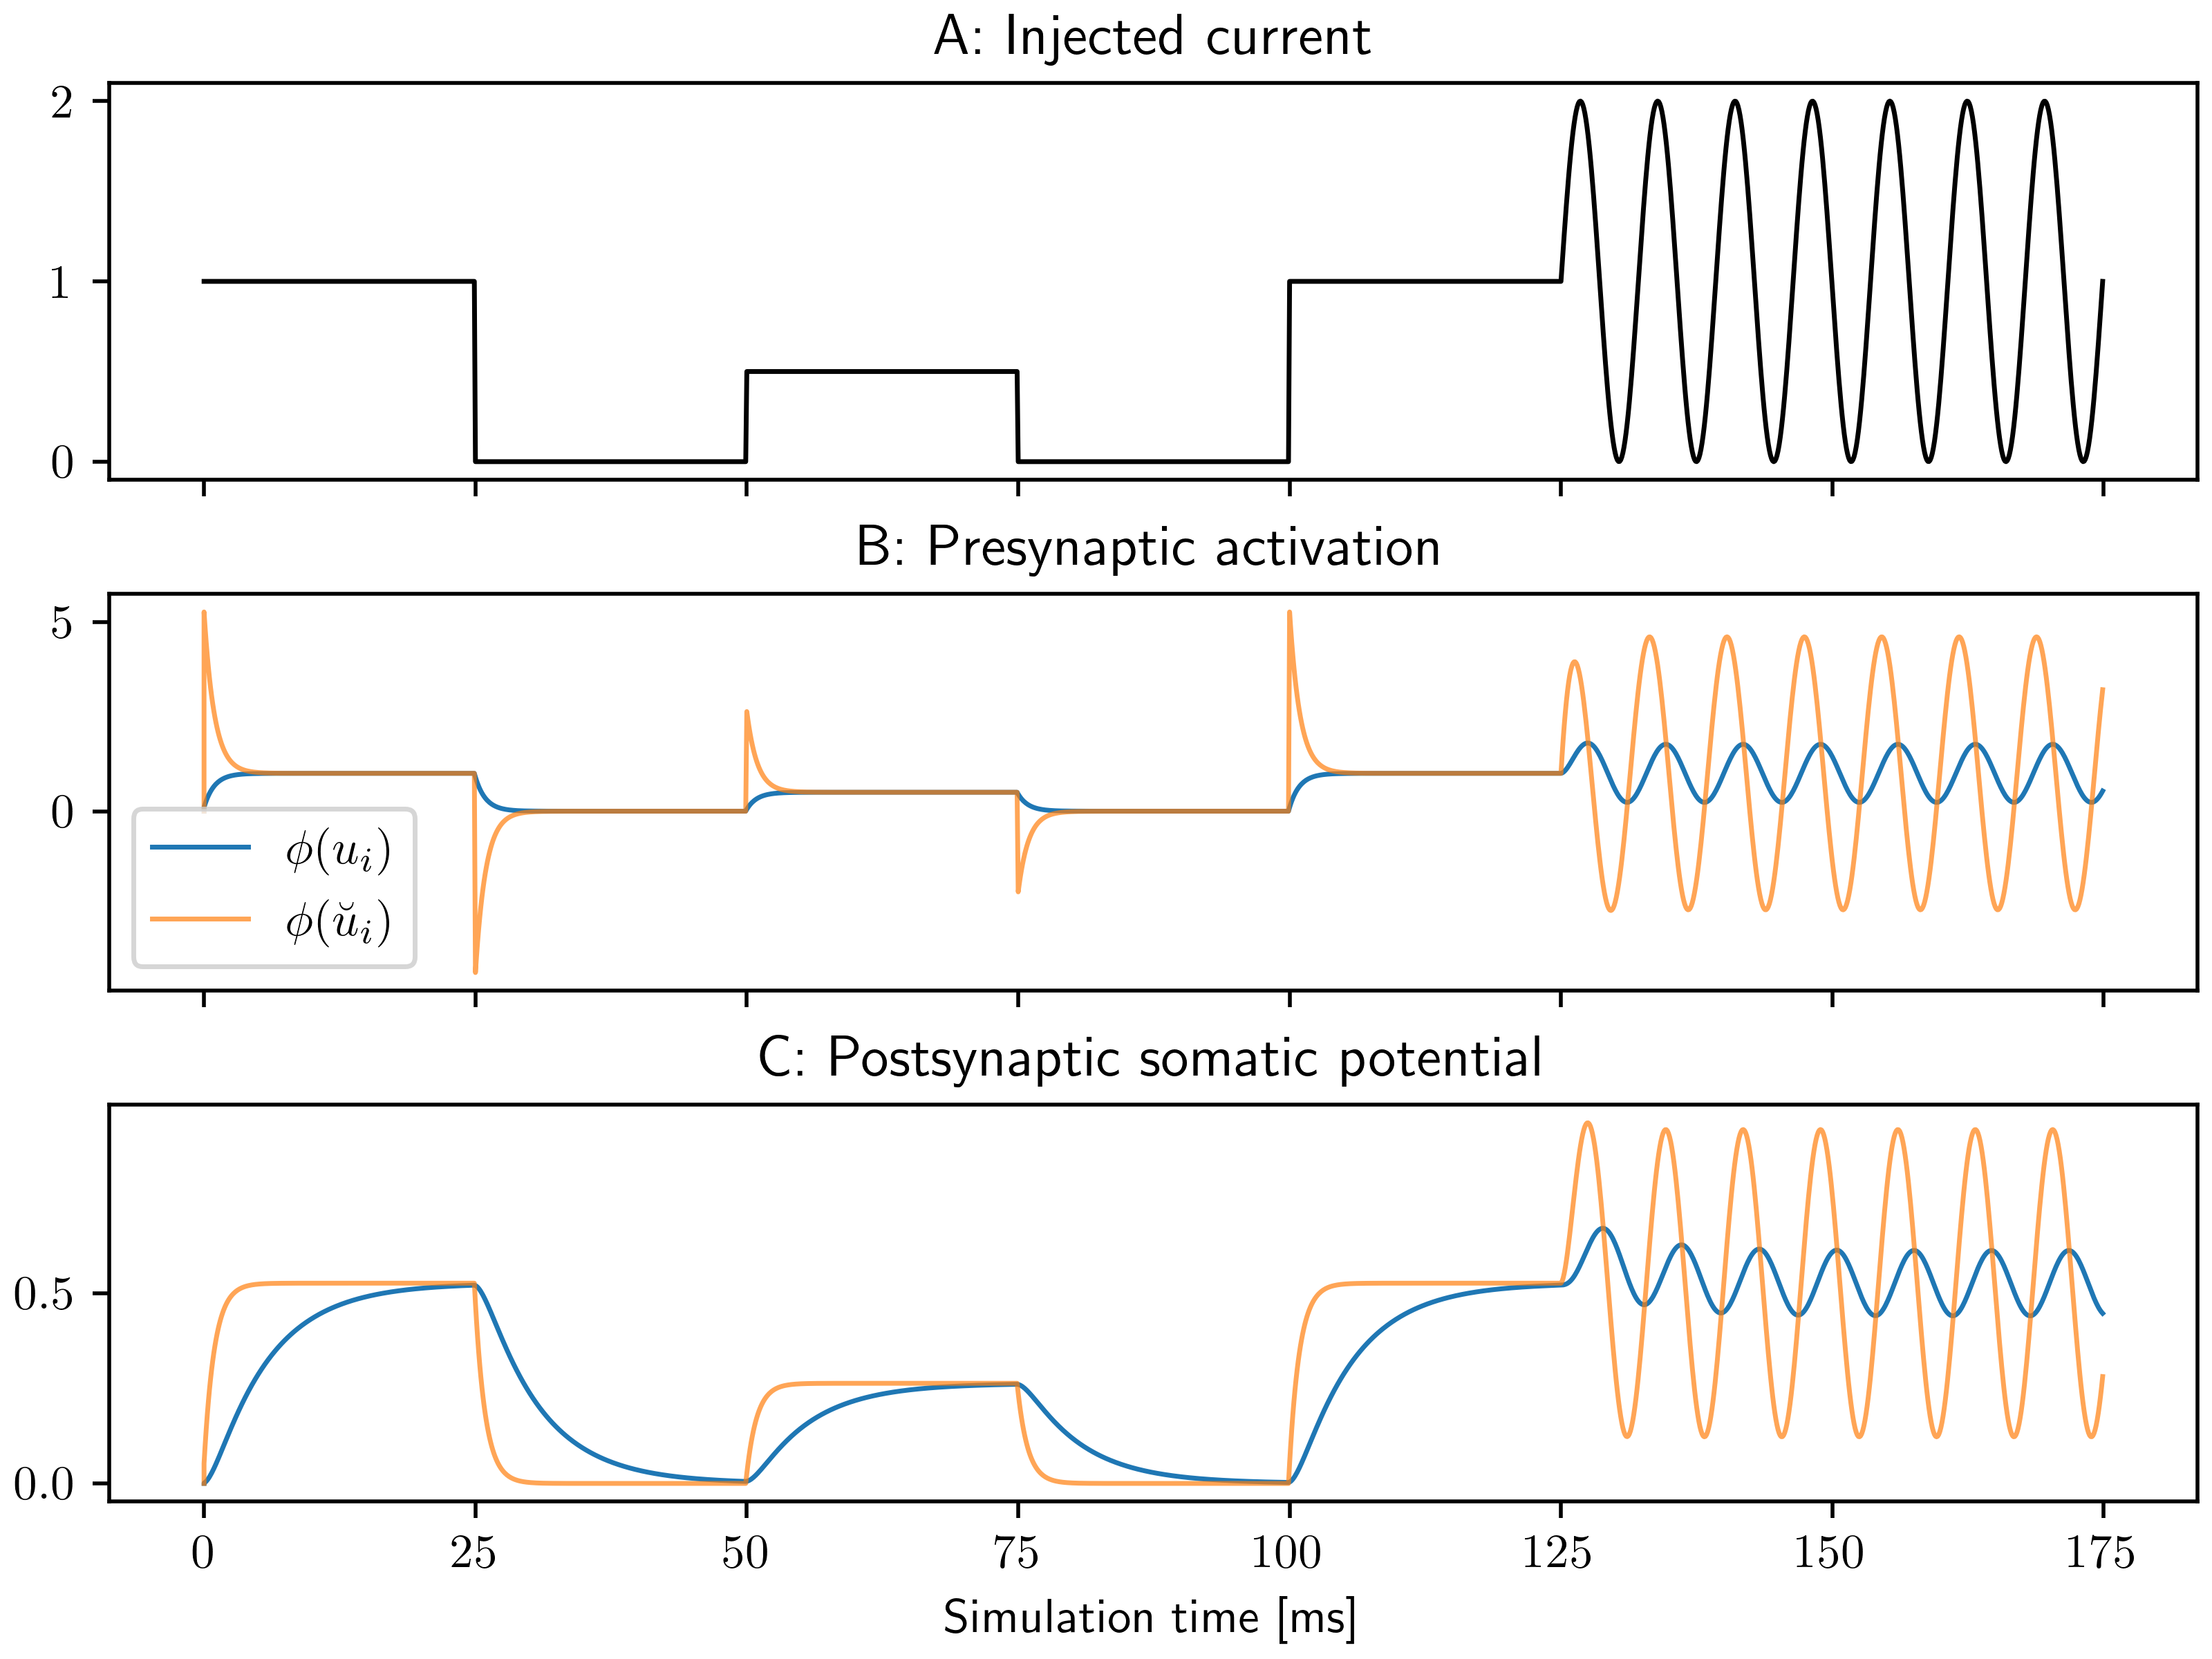
\includegraphics[width=0.8\textwidth]{fig_le_response}
  \caption{Signal transmission between an input neuron $i$ and a hidden layer pyramidal neuron $j$. Depicted are
    activations for the original Sacramento model and prospective activation using Latent Equilibrium. \textbf{A:}
    Current injected into both types of neurons. \textbf{B:} Activation of the input neuron using Sacramento dynamics
    $\phi(u_i)$ (blue), and prospective activation $\phi(\breve{u}_i)$ (orange). Note how strongly prospective
    activation reacts to changes in somatic voltage, leading to jumps in activation. After the input neuron has reached
    its relaxed state ($\dot{u}_i = 0$), both types of neuron evoke the same activation. \textbf{C:} Somatic potential
    $u_j$ of the pyramidal neuron responding to signals sent from the input neuron (color scheme as in B).}
  \label{fig-comparison-le}
\end{figure}

When employing the default parametrization given by Haider et al. \todo{reference parameter table}, $\tau_{eff}$ is
slightly lower than reported pyramidal neuron time constants \citep{McCormick1985} at approximately $5.26ms$. While
employing prospective dynamics does not alter activations and weights at the input layer, neurons at subsequent layers
approach their steady state much more quickly, as depicted in Figure \ref{fig-comparison-le}. This property extends to
the local error terms of pyramidal- and interneurons, which relax much faster for LE networks, as shown in Figure
\ref{fig-error-comp-le}. In the idealized case considered in the original paper, the signal transmission in a
feedforward network is immediate, despite membrane potentials not necessarily catching up. These results highlight the
superiority of LE for learning in this network, as network relaxation is almost instantaneous. In contrast, the error
terms in a Sacramento network drive random synaptic plasticity even when the network is fully trained on a given dataset
and is able to make accurate predictions. Thus, both the issue of redundant weight changes, as well as the concern over
response and learning speed can be solved by LE.\newline




\begin{figure}[h]
  \centering
  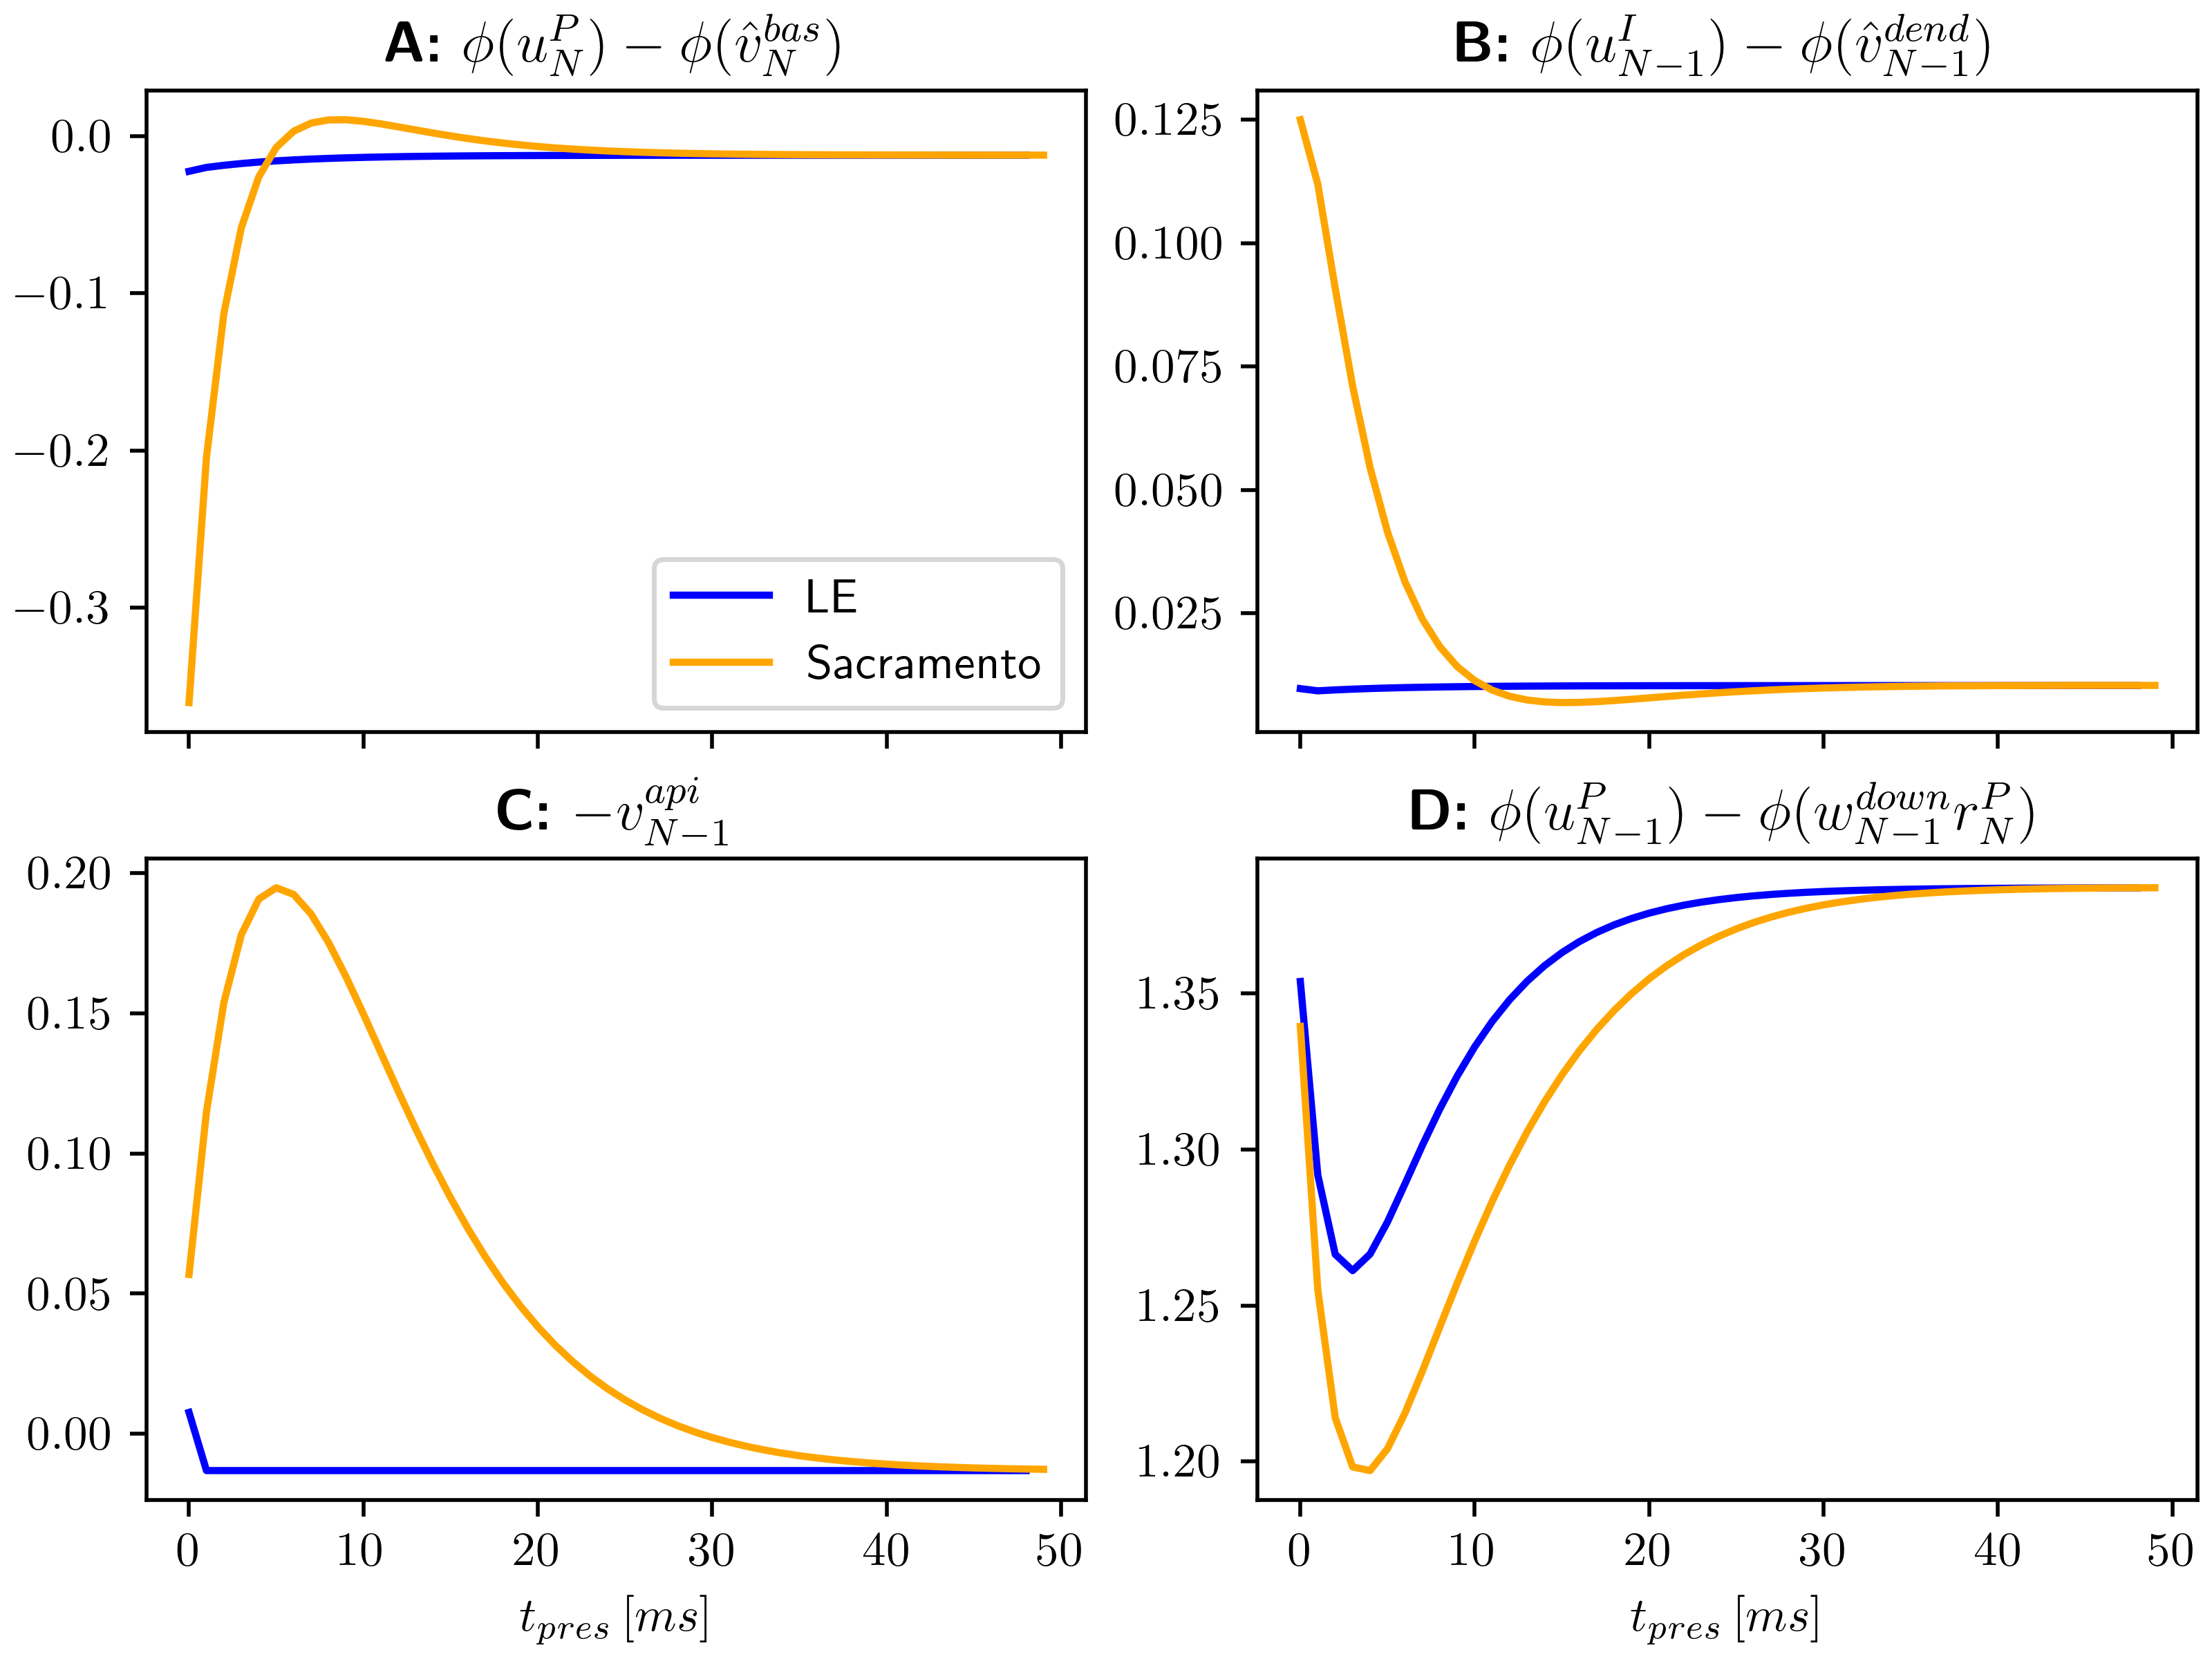
\includegraphics[width=0.9\textwidth]{fig_le_dendritic_errors}
  \caption{Effects of Latent equilibrium on relaxation of the dendritic error terms from Equations
    \ref{eq-delta_w_up}-\ref{eq-delta_w_down}. Depicted are error terms for individual neurons of a network with one
    hidden layer that was fully trained on the Bars dataset \todo{ref}. When employing Sacramento dynamics (orange),
    dendritic errors exhibit longer and more intense deviations, while errors in an identical LE network (blue) relax
    much sooner. Note, that errors do not decay exactly to zero due to the fluctuations inherent to the spiking network
    variant. \textbf{A:} Basal dendritic error for a pyramidal neuron at the output layer. \textbf{B:} Dendritic error
    for a hidden layer Interneuron. \textbf{C:} Proximal apical error for a hidden layer Pyramidal neuron. For this case
    the difference between the two networks is most striking, as errors for the LE network exhibit almost no deviation
    from rest. \textbf{D:} Distal apical error for the same pyramidal neuron. Note that this error term does not
    converge to zero for either network after the relaxation period, an issue that will be discussed in Section
    \ref{sec-feedback-plast}.}
  \label{fig-error-comp-le}
\end{figure}

In addition to using the prospective somatic potential for the neuronal transfer function, it is also used in the
plasticity rule of LE neurons. The Urbanczik-Senn plasticity is therefore updated to compute dendritic error from
prospective somatic activations and a non-prospective dendritic potential $\dot{w}_{ij}= \eta \ (
\phi(\breve{u}_i^{som}) - \phi(\hat{v}_i^{bas}) ) \ \phi(\breve{u}_j^{som})^T$. Much like for the transfer function,
this change serves to increase the responsiveness of the network to input changes. \newline


\todo{keep the following section?}
Besides the using a prediction of future somatic activity for neuronal transfer and plasticity, \cite{Haider2021}
further alter the plasticity rule by means of their implementation. While the simulations by
\cite{sacramento2018dendritic} strictly conforms to the equations above, the new implementation
(\href{https://github.com/neurips}{GitHub}) . The fundamental building block of a network here is a layer, which is
represented in code as an instance of the class \texttt{Layer}. Each instances holds information about its corresponding
pyramidal- and interneurons. It also holds information about the synaptic connections between the two populations, as
well as all incoming feedforward and feedback pyramidal synapses. A layer has two class methods that are fundamental to
its computation; \texttt{update()} computes membrane potential derivatives and synaptic weight changes given pyramidal
neuron activations from the previous and subsequent layers. \texttt{apply()} updates weights and membrane potentials
from the previously calculated changes. Layers are processed in order from input to output layer, where all of them
receive the \texttt{update()} signal first, before \texttt{apply()} is called on all of them. This ordering ensures,
that changes in activation do not cascade through the layers and lead to excessive activations at the output. Yet, since
next layer activations at time $t$ have not been computed, top down information is always delayed by one timestep.
\todo{evaluate importance of this}


Thus, the equations for membrane updates change slightly:

\section{Implementational details}

Building on the neuron and plasticity model from \cite{Stapmanns2021}, a replicate model of the pyramidal neuron with
spiking communication was developed in NEST. The existing Urbanczik-Senn neuron was expanded to three compartments, and
storage and readout of dendritic errors were updated  to allow for compartment-specific plasticity rules. Interneurons
were chosen to be modeled as pyramidal neurons with slightly updated parameters and apical conductance $g^{api}=0$.
Since membrane dynamics of both neurons follow the same principles and additional compartments have minor impact on
performance, this was deemed sufficient.  

After facing some setbacks when attempting to train the first spiking variant of the network, the decision was made to
also implement a rate-based variant of the neuron in NEST.  While the additional effort required for another
implementation might be questionable, this model turned out to be indispensible. It enabled the identification of both
errors in the model, as well as training mechanisms and parameters that required changes to enable spike-compatible
learning.

Following NEST convention, the spiking and rate-based neuron models were named
\texttt{pp\_cond\_exp\_mc\_pyr}\footnote{Despite being somewhat cryptic, the name does actually make sense, as it
describes some key features of the model: It is a \textbf{point process} for \textbf{cond}uctance based synapses and has
an \textbf{exp}onentially decaying membrane in \textbf{multiple compartments}.} and \texttt{rate\_neuron\_pyr}
respectively. Furthermore, the \texttt{pyr\_synapse} class was defined for spike events, and implements a variant of the
event-based Urbanczik-Senn plasticity described in Section \ref{sec-event-urb}. The \texttt{pyr\_synapse\_rate} model on
the other hand transmits rate events and updates its weight according to the original plasticity rule.

Simulations were managed using the python API \texttt{PyNEST} \citep{Eppler2009}, which is much more convenient than the
SLI interface that lies at the core of NEST. An additional advantage of using this language is, that the LE network from
\citep{Haider2021} is also implemented in python. Thus, by including a slightly modified version of that code in my
project, it was possible to unify all three variants in a single network class and accompanying interface. This allowed
for exact alignment of network stimulation and readout and enabled in-depth comparative analyses. In the upcoming
Result, three variants of the same network architecture will therefore be compared; The modified python implementation
from \citep{Haider2021} is termed \texttt{NumPy} based on the framework that is used to compute neuron dynamics and
synaptic plasticity through matrix multiplication. The two NEST variants will be referred to as \textit{NEST spiking}
and \textit{NEST rate}. The NEST rate version will serve to distinguish differences that are due to the novel simulation
backend from those that were introduced by the spike-based communication scheme.

\subsection{Neuron model Adaptations}

The neuron model from \cite{Stapmanns2021} was modified in some ways in order to remove unnecessary parameters and match
the pyramidal neuron implementation more closely. Both the inclusion of nonzero reversal potentials and the flow of
currents from the soma to the dendrites were omitted in my model. \todo{argue?} Furthermore, the present network
requires synapses to be able change the sign of their weight at runtime, which is not permitted in the original synapse
model. For this reason, the strict separation of excitatory and inhibitory synapses had to be removed from the synapse
model. In order to compare the different implementations exactly, the ODE solver with variable stepsize was replaced
with Euler integrations\footnote{This change initially served debugging purposes, but turned out to have no negative
effect on efficiency and was therefore kept} with step size $\Delta t$. For the spiking neuron model, dendritic
compartments are modeled with leaky membrane dynamics in contrast to the rate variant. The choice of dendritic leakage
conductance $g_l^{dend}=\Delta t$ is motivated in Section \ref{sec-gl-dend}. 

A major issue of the spiking network is the fact that under the default parametrization, spikes are too infrequent for
the network to relax quickly and accurately encode dendritic errors. Initial experiments showed that the network is
sensitive to changes in parametrization, which meant that it was desirable to change as few existing parameters as
possible. Therefore, a novel parameter $\psi$ was introduced. In a spiking neuron $i$, the probability of eliciting a
spike is linearly increased by this factor ($r_i = \psi \phi(u_i)$). Likewise, all synaptic weights $W$ in a spiking
network are attenuated by the same factor ($W \leftarrow \frac{W}{\psi}$). These changes cancel each other out, as a
change in $\psi$ elicits no change in absolute compartment voltages of a network. Instead, it serves to stabilize these
voltages over time, which drastically improves learning performance of the network. One mechanism in which this
parameter needs to be considered is the plasticity rule. Weight changes are affected by $\psi$ in three distinct ways:
The dendritic error scales linearly with $\psi$, as does the presynaptic activation. Additionally, since the frequency
of weight changes is determined by the presynaptic spike rate, learning rates are attenuated by $\eta \leftarrow
\frac{\eta}{\psi^3}$. The exception to this are the weights from interneurons to pyramidal neurons, as these do not
depend on dendritic predictions, but on absolute dendritic voltage. Hence, in this case $\eta^{pi}
\leftarrow\frac{\eta^{pi}}{\psi^2}$. On close investigation of the spiking neuron model, one can observe that for $\psi
\rightarrow \inf$, it becomes an exact replication of the rate-based implementation. Unsurprisingly therefore,
increasing $\psi$ caused the spiking network to learn successfully with fewer samples and to a lower test loss. The
argument against increasing $\psi$ is twofold: Initial experiments showed that with $\psi \in [0.5, 1]$, pyramidal and
interneurons exhibit spike frequencies in biologically plausible range of less than $55Hz$
\cite{Kawaguchi2001,Eyal2018}. Additionally, each transmitted \texttt{SpikeEvent} is computationally costly, which
increases training time (cf. Figure \ref{fig-benchmark}) and further makes high spike frequencies undesirable. As a
middle ground, $\psi = 100$ proved useful during initial tests and will be assumed the default from here on out.

With these adaptations, the network was able to perform supervised learning with spiking neurons, as will be discussed
in the upcoming sections.

